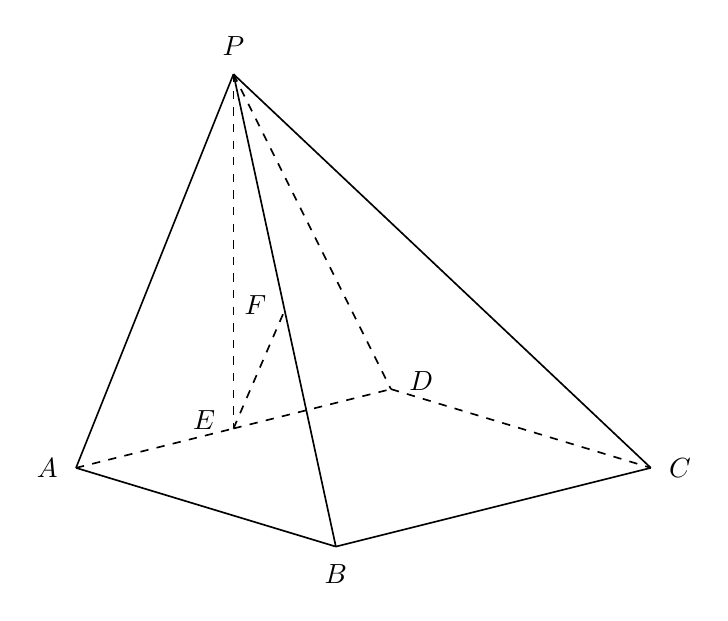
\begin{tikzpicture}[line width=.6pt, font=\normalsize]
% Points (cm, schematic perspective)
\coordinate (P) at (-1.5000000000,5.0000000000);
\coordinate (E) at (-1.5000000000,0.5000000000);
\coordinate (D) at (0.5000000000,1.0000000000);
\coordinate (A) at (-3.5,0.0);
\coordinate (B) at (-0.2,-1.0);
\coordinate (C) at (3.8,0.0);
\coordinate (F) at (-0.8500000000,2.0000000000);
% Solid visible edges
\draw (P) -- (A);
\draw (P) -- (B);
\draw (P) -- (C);
\draw (A) -- (B);
\draw (B) -- (C);
% Hidden / interior dashed edges
\draw[dashed] (P) -- (E);
\draw[dashed] (P) -- (D);
\draw[dashed] (A) -- (E);
\draw[dashed] (E) -- (D);
\draw[dashed] (D) -- (C);
\draw[dashed] (E) -- (F);
% Labels offset to avoid touching strokes
\node[above,yshift=3.0pt] at (P) {$P$};
\node[left,xshift=-3pt] at (A) {$A$};
\node[below,yshift=-3.0pt] at (B) {$B$};
\node[right,xshift=3pt] at (C) {$C$};
\node[left,xshift=-3pt,yshift=3pt] at (E) {$E$};
\node[right,xshift=3pt,yshift=3.0pt] at (D) {$D$};
\node[left,xshift=-3.0pt,yshift=2.0pt] at (F) {$F$};
\end{tikzpicture}
